\documentclass{article}
\usepackage{fontspec}
\usepackage{biblatex}[backend=biber,style=plain]
\usepackage{pgfplots}
\pgfplotsset{compat=1.18}
\usepackage{adjustbox}
\addbibresource{main.bib}
\usepackage{titling}
\usepackage{titlesec}

\setmainfont{Nexus Sans Pro}[Scale=MatchUppercase]
\newfontfamily\headingfont{Nexus Serif Pro}[Numbers=Lining,Scale=MatchUppercase]
\setmonofont{Nexus Typewriter Pro}

\titleformat*{\section}{\LARGE\headingfont}
\titleformat*{\subsection}{\Large\headingfont}
\titleformat*{\subsubsection}{\large\headingfont}
\renewcommand{\maketitlehooka}{\Huge\huge\headingfont}

\title{
    Examination of the Effects of Programming Languages on Developer Productivity, as Measured by Time
}
\author{Ben Raz \texttt{<ben.raz@student.winstonprep.edu>}}
\date{\today}

\begin{document}

\maketitle

\begin{abstract}
    In this study, we test whether programming languages have an effect on developer productivity and how that effect manifests itself by implementing a real-world algorithm in each language. We find that lightweight scripting languages like Python and JavaScript give developers the most productivity while low-level languages like Rust and especially C++ do more to hinder developer productivity. Additionally, we summarize the current literature and discuss the limitations of this study.
\end{abstract}

\section{Introduction}

In one year on earth, developers will spend around 7 billion hours\cite{softwareCodeTime} interacting with a programming language. That is comparable to the lifetime of planets. At this scale, productivity clearly matters. A change of as little as 1\% can free up tens of millions of hours. These hours can go towards fueling innovation. Because of the importance of programmer productivity, we study which popular programming language makes developers the most productive. Additionally, we analyze the tradeoffs of each language. According to both a survey of language popularity\cite{tiobe} and a study analzying the ease of use of writing a string parsing function in a number of different programming languages\cite{prechelt2000}, Python and other scripting languages are prefereable in terms of developer efficiency.

\section{Experimental Design}

The experiment consisted of making a program that organizes files in a directory into sub-folders based on their file type. For example, it would take \texttt{image.png} and change it into \texttt{Png/image.png}. This task requires many things. First, it requires a good standard library as well as robust error handling and string manipulation. It is also similar to real-world work, which is very focused on the filesystem. This program is to be implemented in 5 different languages:


\begin{itemize}
        \item C++
        \item Python
        \item JavaScript
        \item Rust
        \item Java
\end{itemize}

Once the development environement is set up, a stopwatch is started while the software is being written. If, for any reason, a break must occur, the stopwatch is paused and then unpaused as neccessary.Finally, the times are written down in a notes document once development is over. This process repeats for each programming language. 

\section{Results}

The results for each programming language are tabulated below.
\begin{center}
\begin{adjustbox}{center}
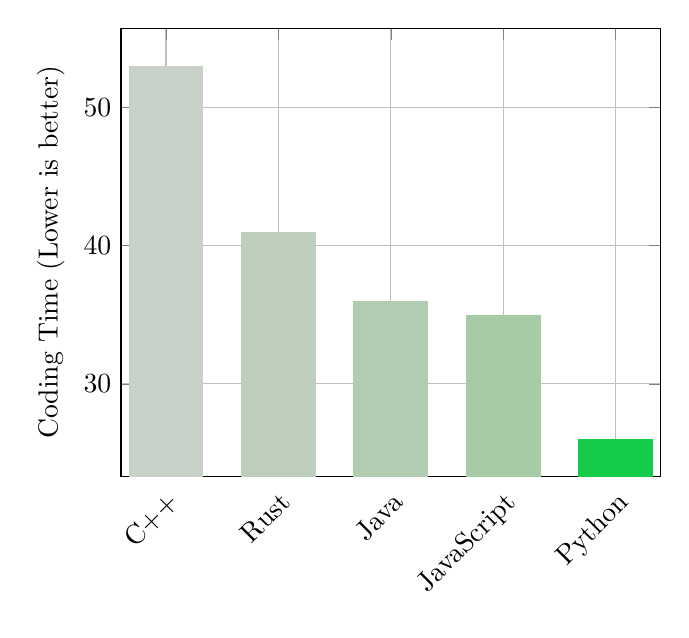
\begin{tikzpicture}
\begin{axis}[
        symbolic x coords={C++,,Rust,,Java,,JavaScript,,Python},
        xticklabel style={rotate=45,anchor=north east},
        xtick={C++,Rust,Java,JavaScript,Python},
        ylabel=Coding Time (Lower is better),
        grid,
        bar width=27pt,
        ]
        \addplot[ybar,draw=none,fill=green!10!gray!40!white] coordinates {(C++, 53)};
        \addplot[ybar,draw=none,fill=green!15!gray!45!white] coordinates {(Rust, 41)};
        \addplot[ybar,draw=none,fill=green!20!gray!50!white] coordinates {(Java, 36)};
        \addplot[ybar,draw=none,fill=green!25!gray!55!white] coordinates {(JavaScript, 35)};
        \addplot[ybar,draw=none,fill=white!10!green!80!blue] coordinates {(Python, 26)};
\end{axis}
\end{tikzpicture}
\end{adjustbox}
\end{center}

According to these results, A winner is clear. Python took only 25 minutes while JavaScript took nearly ten minutes more. Java took 36 minutes while Rust took 41. The C++ implementation took 52 minutes to write, more than twice the time took to write the Python implementation.

\section{Limitations of This Study}

While our findings corroborate similar studies on the topic, we acknowledge the limitations of this study. Firstly, the results may have been distorted by the fact that, for a given person, profficiency varies by the programming language. By only having one person undergo the experiment, we risk generalizing the varied skills of one programmer to the whole industry. Additionally, when choosing a language productivity and ease of coding are rarely the only consideration, which is good. While writing Python is twice as fast as writing C++, no one is seriously considering implementing a database or operating system in Python due to the overwhelming performance differences (Python is almost 200 times slower than C++).
\section{Conclusion}

After testing five different programming languages with a file manipulation program, we conclude, in concordance with the current literature, that high-level interpreted scripting languages like Python generally outperform low-level compiled languages like C++. We further recognize the limitations of the generality of our results, namely small sample size, and reccommend further research consisting of subjects from a wide variety of subproffesions within programming.

\printbibliography


\end{document}
